\documentclass{article}[18pt]
\usepackage{../../../../../format}
\lhead{ADS - Part 4}
\lstset{language=C,
	basicstyle=\ttfamily,
	keywordstyle=\bfseries,
	showstringspaces=false,
	morekeywords={if, else, then, print, end, for, do, while},
	tabsize=4,
	mathescape=true,
	escapechar=£,
	numbers=left,
	stepnumber=1,
}

\usepackage{caption}
\DeclareCaptionFont{white}{\color{white}}
\DeclareCaptionFormat{listing}{\colorbox{gray}{\parbox{\textwidth}{#1#2#3}}}
\captionsetup[lstlisting]{format=listing,labelfont=white,textfont=white}

\begin{document}
\begin{center}
\underline{\huge Depth First Search}
\end{center}
\section{Depth First Search}
\begin{itemize}
	\item Like BFS, DFS explores the graph (but does not find distances to the source)
	\item In contrast to BFS, when a vertex is discovered it is immediately explored
	\item Two timestamps are recorded for each vertex, d and f; the discovery and finish times. We can also record predecessors again
	\item Again colours are used: white for undiscovered, grey for discovered but not finished, black for finished
\end{itemize}
\section{Example}
\begin{center}
	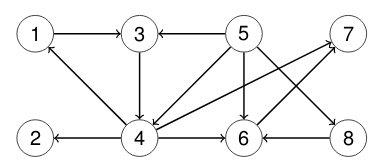
\includegraphics[scale=0.7]{Example}
\end{center}
\begin{itemize}
	\item Initialize: source vertex grey, others white, source discovered at time 1
	\item Repeat
	\begin{itemize}
		\item Increment the time
		\item If there is a white neighbour of the current vertex, then it is coloured grey and its discovery time noted and it becomes current
		\item Else colour the current vertex black, note its finish time and return to its predecessor or jump to an undiscovered vertex, or stop
	\end{itemize}
\end{itemize}
\section{Depth First Search}
\begin{lstlisting}[caption=DFS(G)]
for each vertex $u\in V[G]$
	do colour[u]$\leftarrow$WHITE
		$\pi[u]\leftarrow$ NIL
time $\leftarrow$ 0
for each vertex $u\in V[G]$
	do if colour[u]=WHITE
		then DFS-VISIT(u)
\end{lstlisting}
\begin{lstlisting}[caption=DFS-VISIT(u)]
colour[u]$\leftarrow$ GREY £\hfill£ [vertex u has just been discovered]
time$\leftarrow$time+1
d[u]$\leftarrow$time
for each vertex $v\in$ Adj[u] £\hfill£ [explore edge (u,v)]
	do if colour[v]=WHITE
		then $\pi[v]\leftarrow u$
			DFS-VISIT(v)
colour[u]$\leftarrow$BLACK £\hfill£ [u has been processed]
f[u]$\leftarrow$time$\leftarrow$time+1
\end{lstlisting}
\section{Analysis}
\begin{itemize}
	\item Initialisation takes time $\mathcal{O}(V)$
	\item Time $\mathcal{O}(V)$ is spent on incrementing time, colouring vertices and updating d and f
	\item Each vertex in each adjacency list is considered at most once. This takes time $\mathcal{O}(E)$
	\item Total time is $\mathcal{O}(V+E)$
\end{itemize}
The edges used for discovering new vertices from the depth first tree (or forest). Again we can find this with a predecessor array
\section{Example}
\begin{center}
	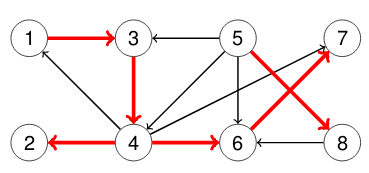
\includegraphics[scale=0.7]{Example1}
\end{center}
Once we have run DFS on a graph we can construct the predecessor subgraph. This has the same vertex set as the graph, and for each vertex v there is an edge from the predecessor of v to v\\
\\
The predecessor subgraph is a depth first forest
\section{Classification of the edges}
Once we have obtained a DFS-Forest for the graph G, we can classify the edges of G
\begin{itemize}
	\item Tree edges are those edges in the DFS-Forest
	\item Back edges are edges that join a vertex to an ancestor 
	\item Forward edges are edges not in the tree that join a vertex to its descendant
	\item Cross edges: all other edges
\end{itemize}
\section{Example}
\begin{center}
	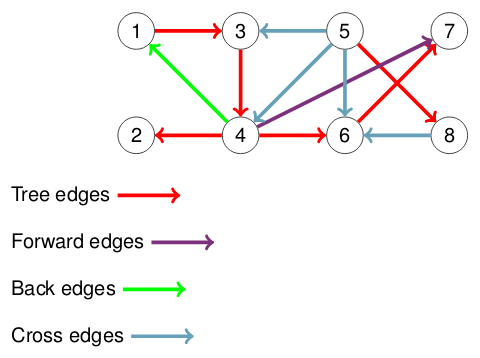
\includegraphics[scale=0.7]{Example2}
\end{center}
\section{Classification of the edges}
The classification is ambiguous for undirected graphs (back edges and forward edges are the same thing)
\begin{itemize}
	\item e is a forward edge if DFS first consideres e from u
	\item e is a back edge if DFS first considers e from v
\end{itemize}
\subsection{Theorem}
In an undirected graph, every edge is a tree edge or a back edge
\section{Using DFS}
\begin{center}
	\includegraphics[scale=0.7]{"Using DFS"}
\end{center}
\begin{itemize}
	\item Every edge in an undirected graph is either a tree edge or a black edge
	\item A graph is connected if each pair of vertices is joined by a path
	\item A cycle is a sequence of edges that start and end at the same vertex
	\item An articulation point is a vertex whose removal disconnects the graph
\end{itemize}
Can we adapt DFS to obtain algorithms that
\subsection{Check whether a graph is connected}
$\mathcal{O}(V+E)$\\
Amend DFS to prevent jumping to undiscovered vertices (don't jump to undiscovered vertex if no more connected ones available)\\
Run DFS with an arbitrary source\\
The graph is connected $\Leftrightarrow$ DFS finds all vertices
\subsection{Discover a cycle in a graph}
$\mathcal{O}(V+E)$\\
Run DFS with an arbitrary source\\
The graph contains a cycle $\Leftrightarrow$ a back edge is discovered during DFS
\subsection{Find all the articulation points in a graph}
$\mathcal{O}((V+E)V)=\mathcal{O}(V^3)$\\
For each vertex u\\
Remove u from the graph\\
Run DFS on the new graph from any source\\
$u$ is an articulation point $\Leftrightarrow$ the new graph is not connected
\subsubsection{Alternate method}
Run DFS once\\
Can we recognise the articulation points?\\
The \textbf{source} is an articulation $\Leftrightarrow$ the source has more than one child in the depth first tree\\
\\
\textbf{Leaves} don't need checking as they are not connected\\
\\
\textbf{Other vertices}: a vector u is an articulation point unless there is a back edge from every child subtree to the parent subtree
\subsubsection{One run method}
Remember back edges - which ones most useful/important\\
Back edges in a chain of nodes mean that removing the nodes below that edge doesn't disconnect a graph\\
Create an array that records, for each vertex v, the most distant ancestor to which there is a back edge\\
In fact, we want the most distant ancestor from which there is a back edge from either v or one of its descendants\\
\\
Create an empty array N\\
Let N[v]=v\\
Run DFS and update N to record the most distant ancestor connected by a back edge to v or its descendants.
\end{document}
